\subsection{Defining Scope}


Goal is to capture the largest computationally feasible network with a simple set of rules. 

The first rule was to restrict the network to ``inner london''. This has the advantage of a formal designation by the GLA for each borough, capturing, XXX\% of the population with a population density of XXXXXX compared to XXXXX for london overall, XXXXXX\% of the jobs in the city, and XXXX\% of the journey's to work. Additionally, rates of cycling are higher in inner London than in the periphery. 

Second, the area of interest was restricted to north of the river Thames. This captures XXX\% of the population, with a density of XXXXXXX, XXX\% of London's jobs, and XXX\% of the journey's to work. Further, it has the advantage of excluding the need to cross the river, where journey's are focused on a few number of bridges, with a significant effect on the shortest paths, reducing the effect of other changes on the network. 

\begin{table}[]
\centering
\begin{tabular}{lcccl}
 Mode Share Within Scope & All Modes & Bicycle & \% by bicycle &  \\
 \hline
 Origin in scope &  981,354 & 46,832 & 4.8\% &  \\
 Destination in scope & 1,454,606 & 48,461 & 3.3\% &  \\
 Both in scope & 479,882 & 24,843 & 5.2\% & \\
 All journeys & 5,852,298 & 140,180 & 2.4\% \\ 
\end{tabular}
\caption{commuter data}
\label{table:commute_data}
\end{table}

text

\subsection{Defining Networks}


\subsubsection{London's OSM data}

\subsubsection{Filters used}

\begin{figure}
  \centering
  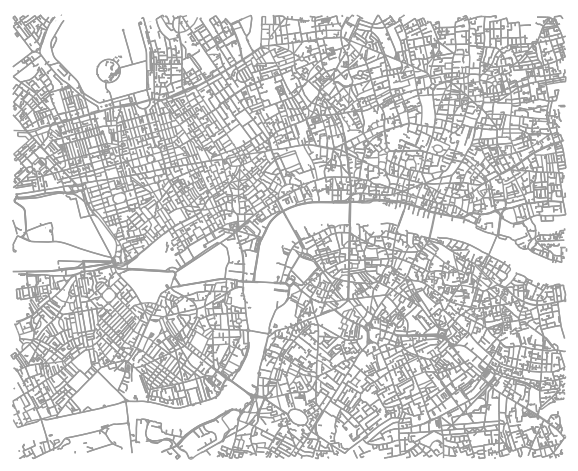
\includegraphics[width=0.5\linewidth]{bbox_bike_1_filter_cropped}
  \caption{1: most confident cyclists}
  \label{fig:sub1}
\end{figure}

\begin{figure}
  \centering
  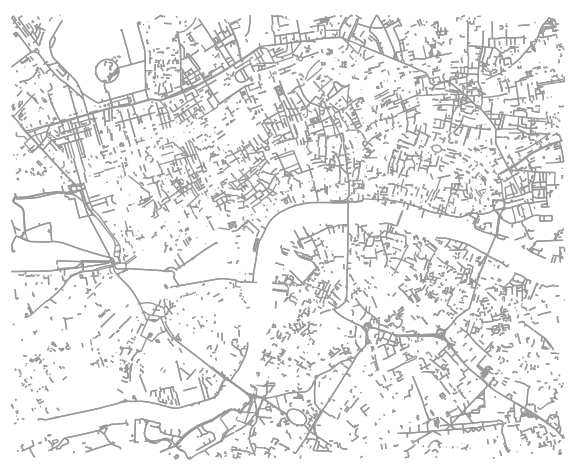
\includegraphics[width=0.5\linewidth]{bbox_bike_5_filter_cropped}
  \caption{5: no interaction with cars }
  \label{fig:sub2}
\end{figure}


\subsubsection{Quant Network}



\subsection{Network Characteristics}

\begin{table}
\centering
\caption{table of network statistics}
\label{table:network_stats}
\end{table}

\subsection{Defining Origins and Destinations}

\begin{figure}
\centering
\caption{distribution of differences between Quant distances and Cycle Origins and Destinations}
\label{fig:diff_dist}
\end{figure}

\subsection{Travel Times}

Travel times were converted from distances using a walking speed of 3 mph and a cycling speed of 8 mph based on data taken from google maps estimates for journeys as seen in that table. 

\begin{table}
\centering
\caption{google speed estimates}
\label{table:google_speeds}
\end{table}


\begin{table}
\centering
\caption{travel time statistics}
\label{table:travel_time_stats}
\end{table}

\subsection{Changes in Routing}


\subsubsection{compare route across directedness}
\begin{figure}
\centering
\caption{example of routing on directed network 1}
\label{fig:routing_1}
\end{figure}

\begin{figure}
\centering
\caption{example of routing on undirected network 1}
\label{fig:routing_1}
\end{figure}

\subsubsection{compare route across level 1 and 2}

\begin{figure}
\centering
\caption{example of routing on directed network 1}
\label{fig:routing_1}
\end{figure}

\begin{figure}
\centering
\caption{example of routing on directed network 2}
\label{fig:routing_1}
\end{figure}

\subsubsection{compare across level 2 directedness}

\begin{figure}
\centering
\caption{example of routing on directed network 2}
\label{fig:routing_1}
\end{figure}

\begin{figure}
\centering
\caption{example of routing on undirected network 2}
\label{fig:routing_1}
\end{figure}


\subsection{Accessibility}

\begin{figure}
\centering
\caption{lsoas colored by directness of routes to other lsoas}
\label{fig:lsoa_directness}
\end{figure}

\subsection{notes on computation}


% table for computation times across algorithm types

% table for computation times across network types
%\begin{table}[]
%\centering
%\begin{tabular}{lllll}
%network  & 1 & 1 undirected & 2  & 2 undirected   \\
%time     & 24:00   & 72:00??  & 9:03  & 36:00        \\        
%\end{tabular}
%\caption{Computation Times}
%\label{table:1}
%\end{table}

\begin{table}[]
\centering
\begin{tabular}{@{}l|llll@{}}
network     & 1           & 1 undirected & 2    & 2 undirected \\ \hline
time(hours) & $\sim$24:00 & $\sim$72:00  & 9:03 & $\sim$36:00 
\end{tabular}
\caption{Calculation times for routes}
\label{table:net_calc_times}
\end{table}

\begin{table}
\centering
\caption{computation times using different algorithms}
\label{table:comp_times_algo}
\end{table}


text